\NextFile{NetworkEditor.html}
\section{networkEditor}

\subsubsection{Starting the network editor}

If you're working with a release, make sure to have MATSim and the networkEditor extension \href{http://www.matsim.org/downloads}{downloaded}.
\begin{itemize}
	\item \textbf{If you use Eclipse to run MATSim}
\\     Make  sure that you have MATSim correctly added to your project's build path.  Add the jar file for the networkEditor the same way to your project's  build path. Then, start the class 
\texttt{org.matsim.contrib.networkEditor.run.NetworkEditor}.
	\item \textbf{If you run MATSim on a shell / command line}
\\      Make sure you have MATSim correctly downloaded and ready for use. Add  the networkEditor extension next to the MATSim jar file and the 
\texttt{libs} directory. Then, use the following command to start the network editor:
\\
\texttt{java -Xmx512m -cp networkEditor/networkEditor.jar:matsim.jar $\backslash$
\\      org.matsim.contrib.networkEditor.run.NetworkEditor}
\\Note: On Windows, use 
\texttt{;} instead of 
\texttt{:} to separate the two jar files.
\end{itemize}

Depending on the size of the network you want to edit, make sure  the editor has enough memory by increasing the memory limit (e.g. "
\texttt{-Xmx1500m}" instead of only "
\texttt{-Xmx512m}").

If the application correctly starts, you should see window similar to the one below:

\begin{figure}[htp]
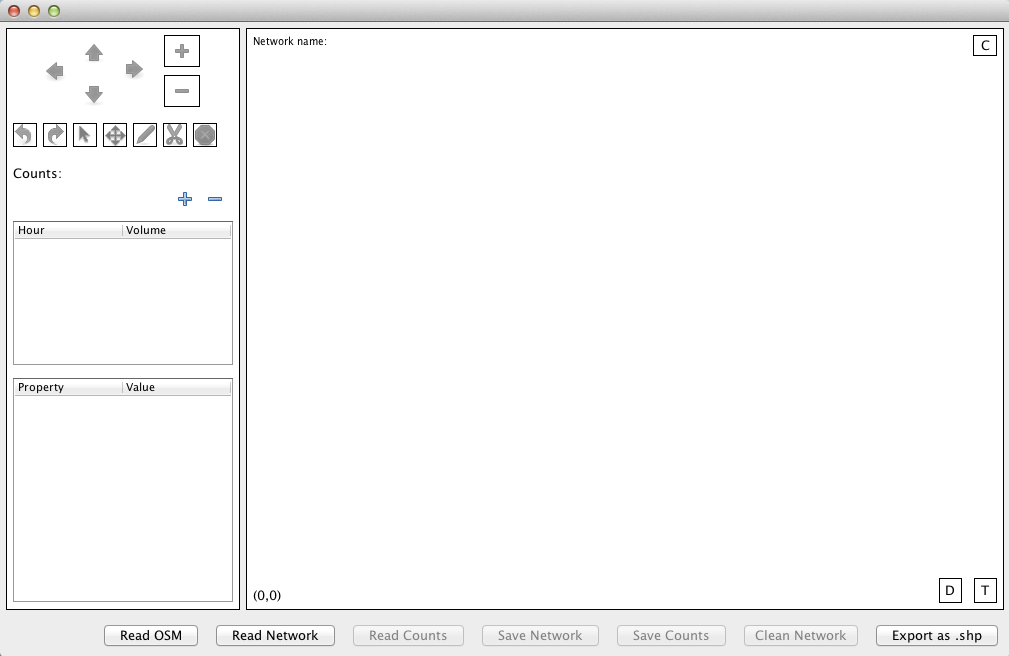
\includegraphics[width=\textwidth]{figures/networkEditor/emptyNetworkEditor.png}
\end{figure}

\subsubsection{Loading network data}

To load an existing MATSim network, click on the button "Read  Network" at the bottom of the window and select the network you want to  load.

Alternatively, you can import data from OpenStreetMap (OSM) and  automatically convert it into a network. For this, first download the  osm data for the region you're interested in. The \href{http://www.matsim.org/docs/tutorials/8lessons/input/creating/network}{tutorial}  contains information on how you can download the required data from  OSM. Once you have a *.osm file containing the data for your region,  click on the button "Read OSM" and select the file. When loading the  data, the following window will open:


\begin{figure}[htp]
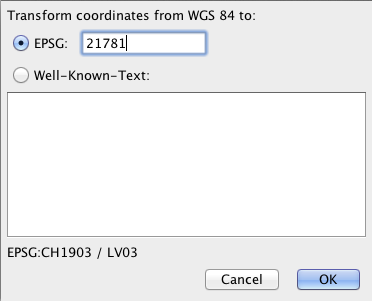
\includegraphics[width=0.6\textwidth]{figures/networkEditor/crsNetworkEditor.png}
\end{figure}

The original data from OSM contains coordinates in the WGS 84  coordinate reference system. WGS 84 is impractical to work with in  MATSim, so we need to convert the coordinates into another coordinate  reference system (CRS). In the example above, we convert it to the Swiss  national coordinate reference system. To find the corresponding EPSG  codes, or the Well-Known-Text description of your CRS, have a look at \href{http://spatialreference.org/}{http://spatialreference.org/} and search for your CRS.

Click OK to close the dialog once you have the correct CRS set. The  OSM data will now be converted and the network displayed afterwards in  the editor. Especially for larger osm files, have some patience for the  conversion process. It may take some while to convert the data and  finally show the network.

\subsubsection{Editing network}

Once a network is loaded, most of the tools in the upper left corner of the window become active:

\begin{figure}[htp]
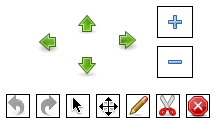
\includegraphics[width=.5\textwidth]{figures/networkEditor/toolsNetworkEditor.png}
\end{figure}

The 4 green arrows are to move the network around in the editor view.  The blue + and – are for zooming in and out. In the row below, the  buttons have the following functionality:
\begin{itemize}
	\item undo / redo: revert and redo changes you did to the network
	\item Selection: select a link or a node by clicking on them in the editor  view. click and drag to select multiple elements. If you have a single  link selected, you can change some of the link's attributes in the panel  on the lower left of the window.
	\item move view: click and drag the network to move the network in the editor view
	\item add link: click in a place to start a new link, click a second time  to end the link at that place. If the clicks are close to a node, the  link will start/end at that node, otherwise a new node will be created.
	\item divide a link: select a link first, then use the scissors to cut the  link into two. A new node will be added at the location of the click,  and the original link will be splitted into two parts.
	\item delete a link: select a link first, then click this button to delete  the selected link. If you clicked on the button by accident, use the  undo-button.
\end{itemize}

\subsubsection{Saving a network}

To save a network in MATSim's format, click on the button "Save  Network". Alternatively, you can export the network as a Shape file that  can be used by allmost all GIS applications for visualization purposes  (but not necessarily for network operations that some GIS applications  offer). Just click on "Export as Shp" to export the network as a Shape  file.

\subsubsection{Working with counts data}

Once you have a network loaded, you can optionally also load some  existing counts for this network. If you just converted your network  from OSM data, you likely won't have any such file. In that case, you  can directly start to add counts where you want. Select a link by  clicking on it. If the link already has counts associated, they will be  displayed in the panel on the left side of the window. Click the + there  to add count values, even if no counts exist yet for this link.

After you're done with the counts editing, save the counts to a file by clicking on "Save Counts".
